For clear skies, two approaches to determine the optimal orientation angle $\gamma_{c}$ (surface azimuth angle) and inclination angle $\beta_{opt}$ are shown in \citemarsenv{Appelbaum1993}. Equation \ref{eq:optimal_beta_irradiance} is described as a ``coarse approximation'' in \citeother{Soulayman2016} and gives $\beta_{opt}$ based on the direct beam irradiance at noon:

\begin{equation}
  \label{eq:optimal_beta_irradiance}
  \beta_{p} = \phi - \delta_{p}
\end{equation}

where $\beta_{p}$ is the optimal inclination angle for a period $p$, $\phi$ is the planetary latitude, and $\delta_{p}$ is the average declination angle for the period $p$.

A ``better approximation'' is shown in \citemarsenv{Appelbaum1995} based on the daily beam insolation on the surface from sunrise to sunset. However, comparing the results using this method to those obtained with Equation \ref{eq:optimal_beta_irradiance} suggest a sign error in the published formula which has been rectified in Equation  \ref{eq:optimal_tanbeta_insolation}:

\begin{equation}
  \label{eq:optimal_tanbeta_insolation}
  \tan{\beta} = -\frac{\cos{\omega_{sr}}\sin{\phi}\cos{\delta}-\left[1-\left(\frac{2\omega_{sr}}{\pi}\right)^{2}\right]\cos{\phi}\sin{\delta}}{\cos{\omega_{sr}}\cos{\phi}\cos{\delta}+\left[1+\left(\frac{2\omega_{sr}}{\pi}\right)^{2}\right]\sin{\phi}\sin{\delta}}
\end{equation}


where $\omega_{sr}$ is the sunrise hour angle. The sign error correction is not necessary for $L_{s} = \SI{180}{\degree}$, as shown in Equation \ref{eq:optimal_tanbeta_insolation_Ls180}.

\begin{equation}
  \label{eq:optimal_tanbeta_insolation_Ls180}
  \tan{\beta_{L_{s} = \SI{180}{\degree}}} = \frac{\cos{\omega_{sr}}\sin{\phi}\cos{\delta}-\left[1-\left(\frac{2\omega_{sr}}{\pi}\right)^{2}\right]\cos{\phi}\sin{\delta}}{\cos{\omega_{sr}}\cos{\phi}\cos{\delta}+\left[1+\left(\frac{2\omega_{sr}}{\pi}\right)^{2}\right]\sin{\phi}\sin{\delta}}
\end{equation}

For both cases, $\gamma_{c} = \SI{0}{\degree}$, that is the inclined surface faces the equator (i.e. oriented South when located in the Northern hemisphere and oriented North when located in the Sourthern hemisphere).




\begin{figure}[h]
\vspace{-2ex}
\centering
    %% setup sizes
    \setlength{\subfigureWidth}{0.50\textwidth}
    \setlength{\graphicsHeight}{80mm}
    %% kill hyper-link highlighting
    \hypersetup{hidelinks=true}%
    %% the figures
    \begin{subfigure}[t]{\subfigureWidth}
        \centering
            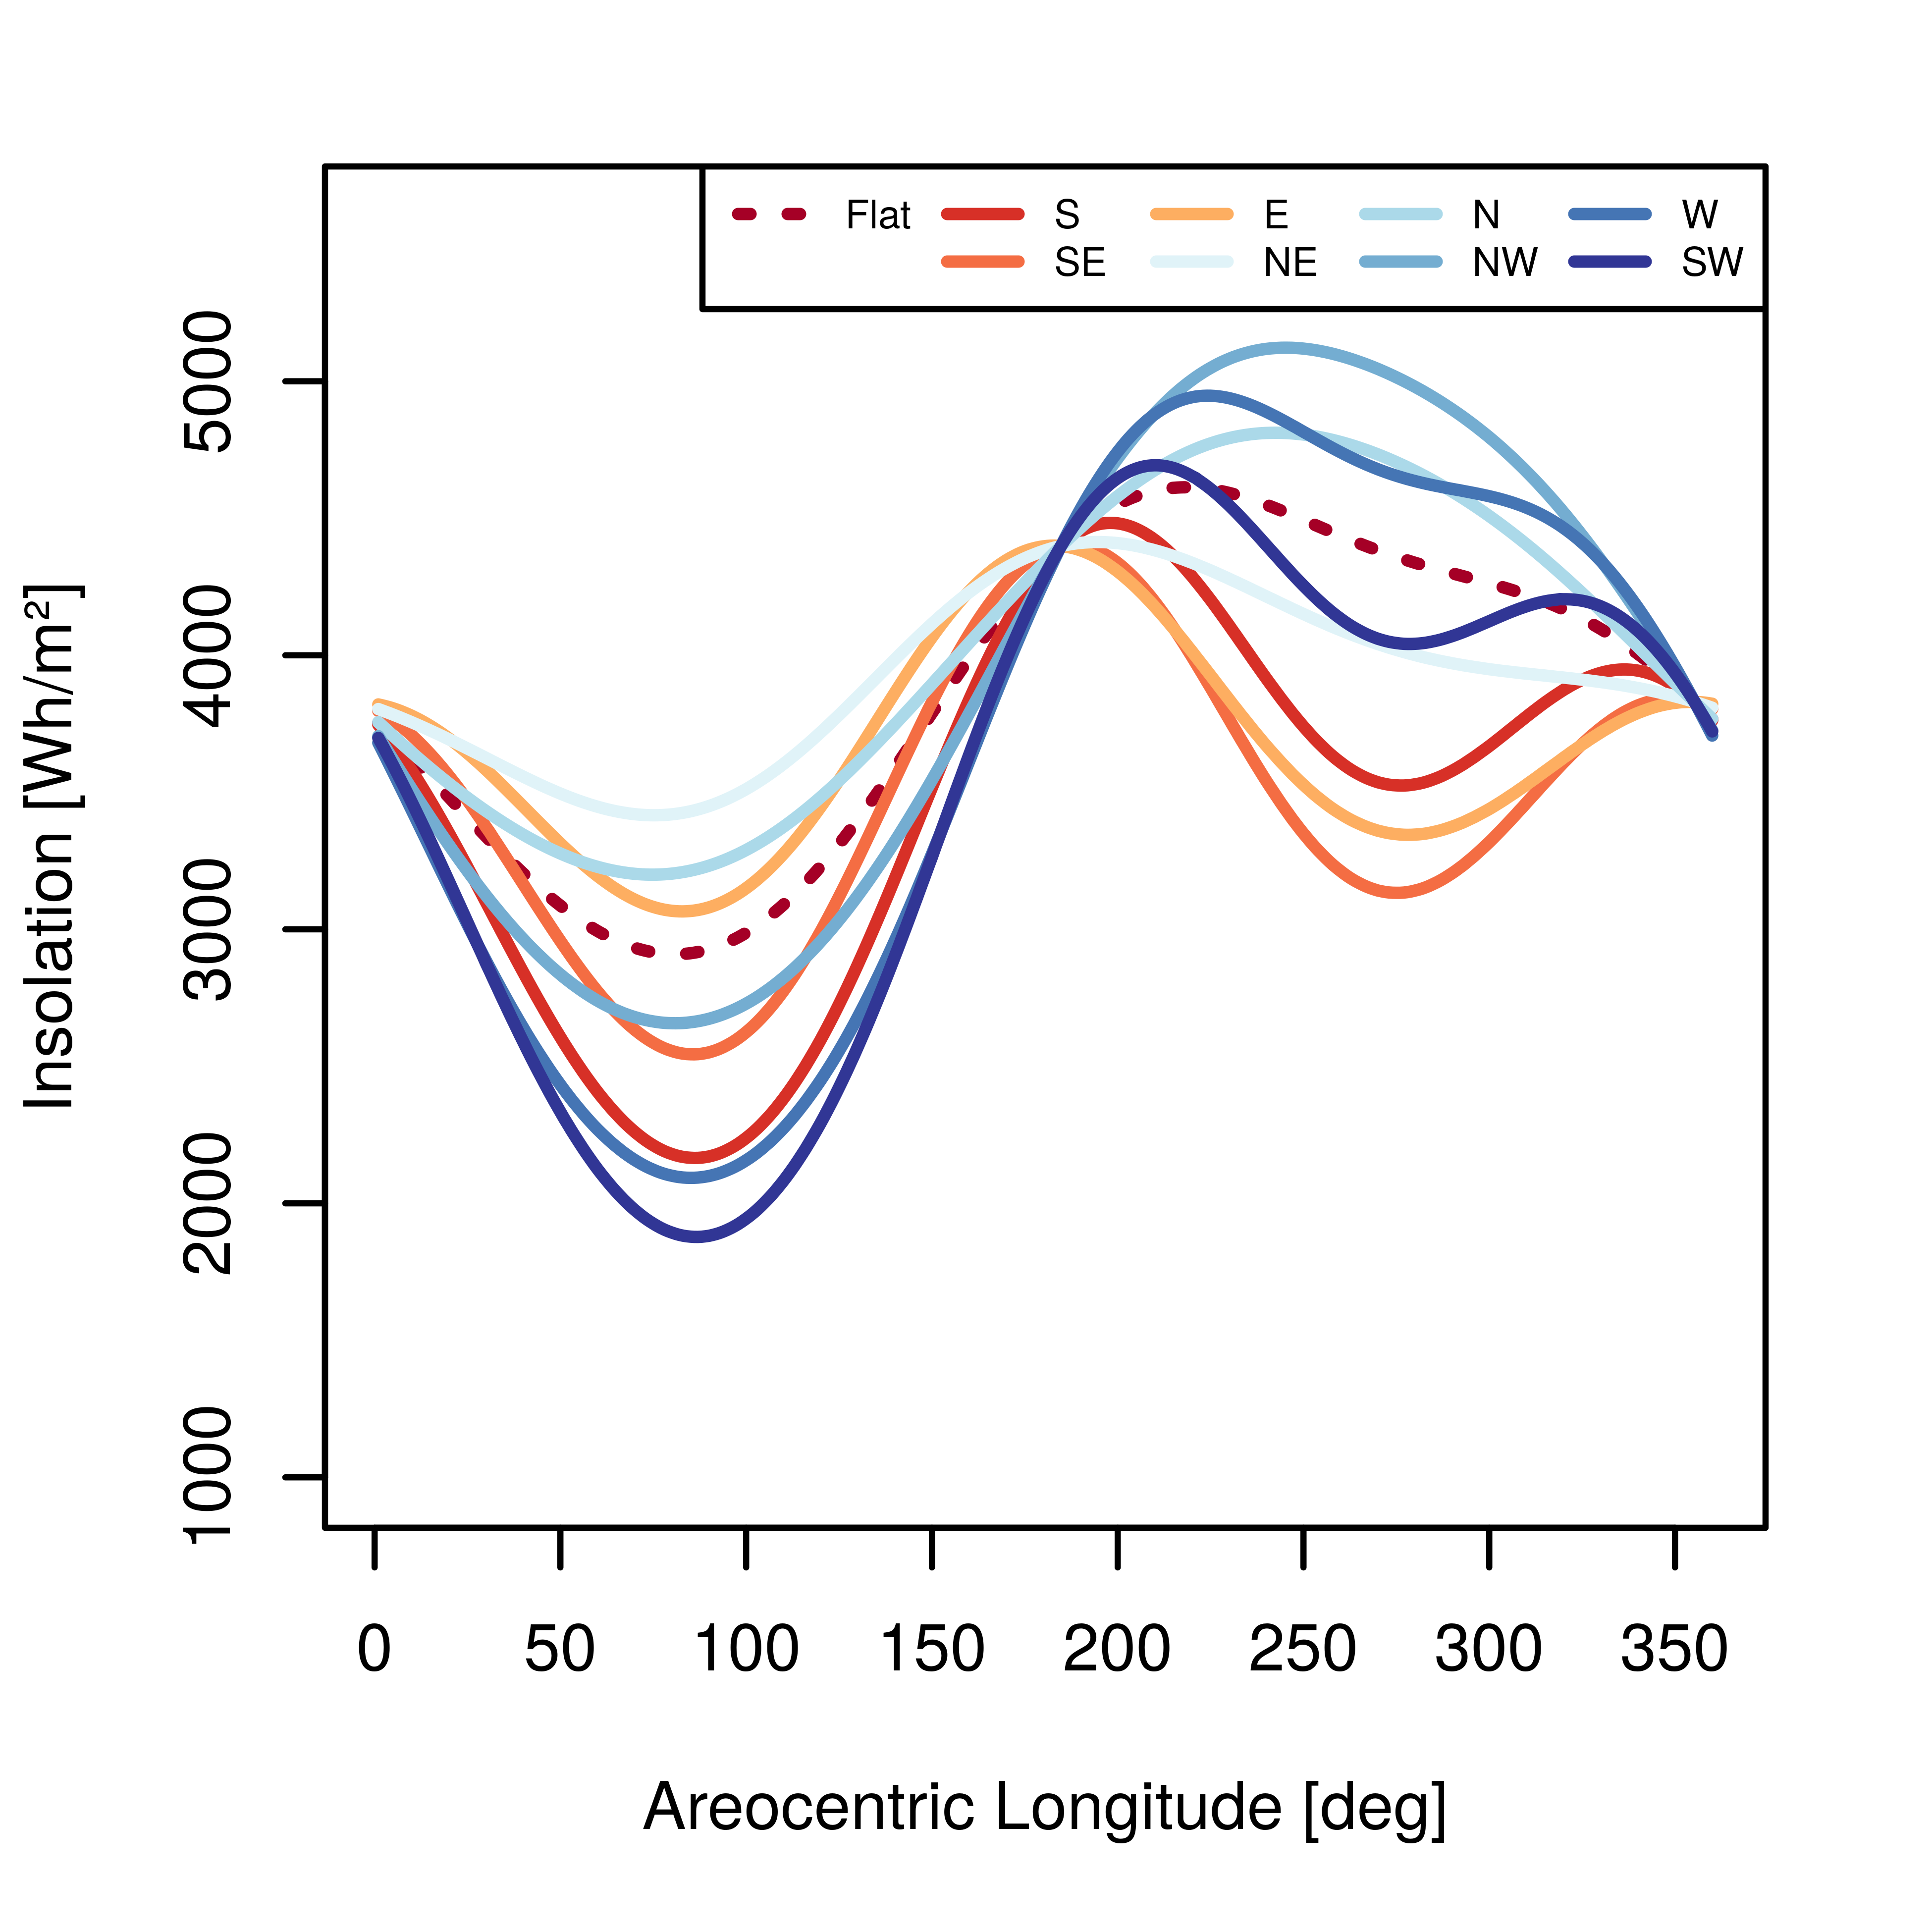
\includegraphics[height=\graphicsHeight]{sections/appendix/optimal-angles/plots/iani-chaos-tau-04-and-beta-optimal-based-on-direct-beam-irradiance-at-noon.png}
            \subcaption{Based on the direct beam irradiance at noon.}
            \label{fig:sub:optimal-angles-iani-chaos-based-on-irradiance}
    \end{subfigure}\hfill
    \begin{subfigure}[t]{\subfigureWidth}
        \centering
            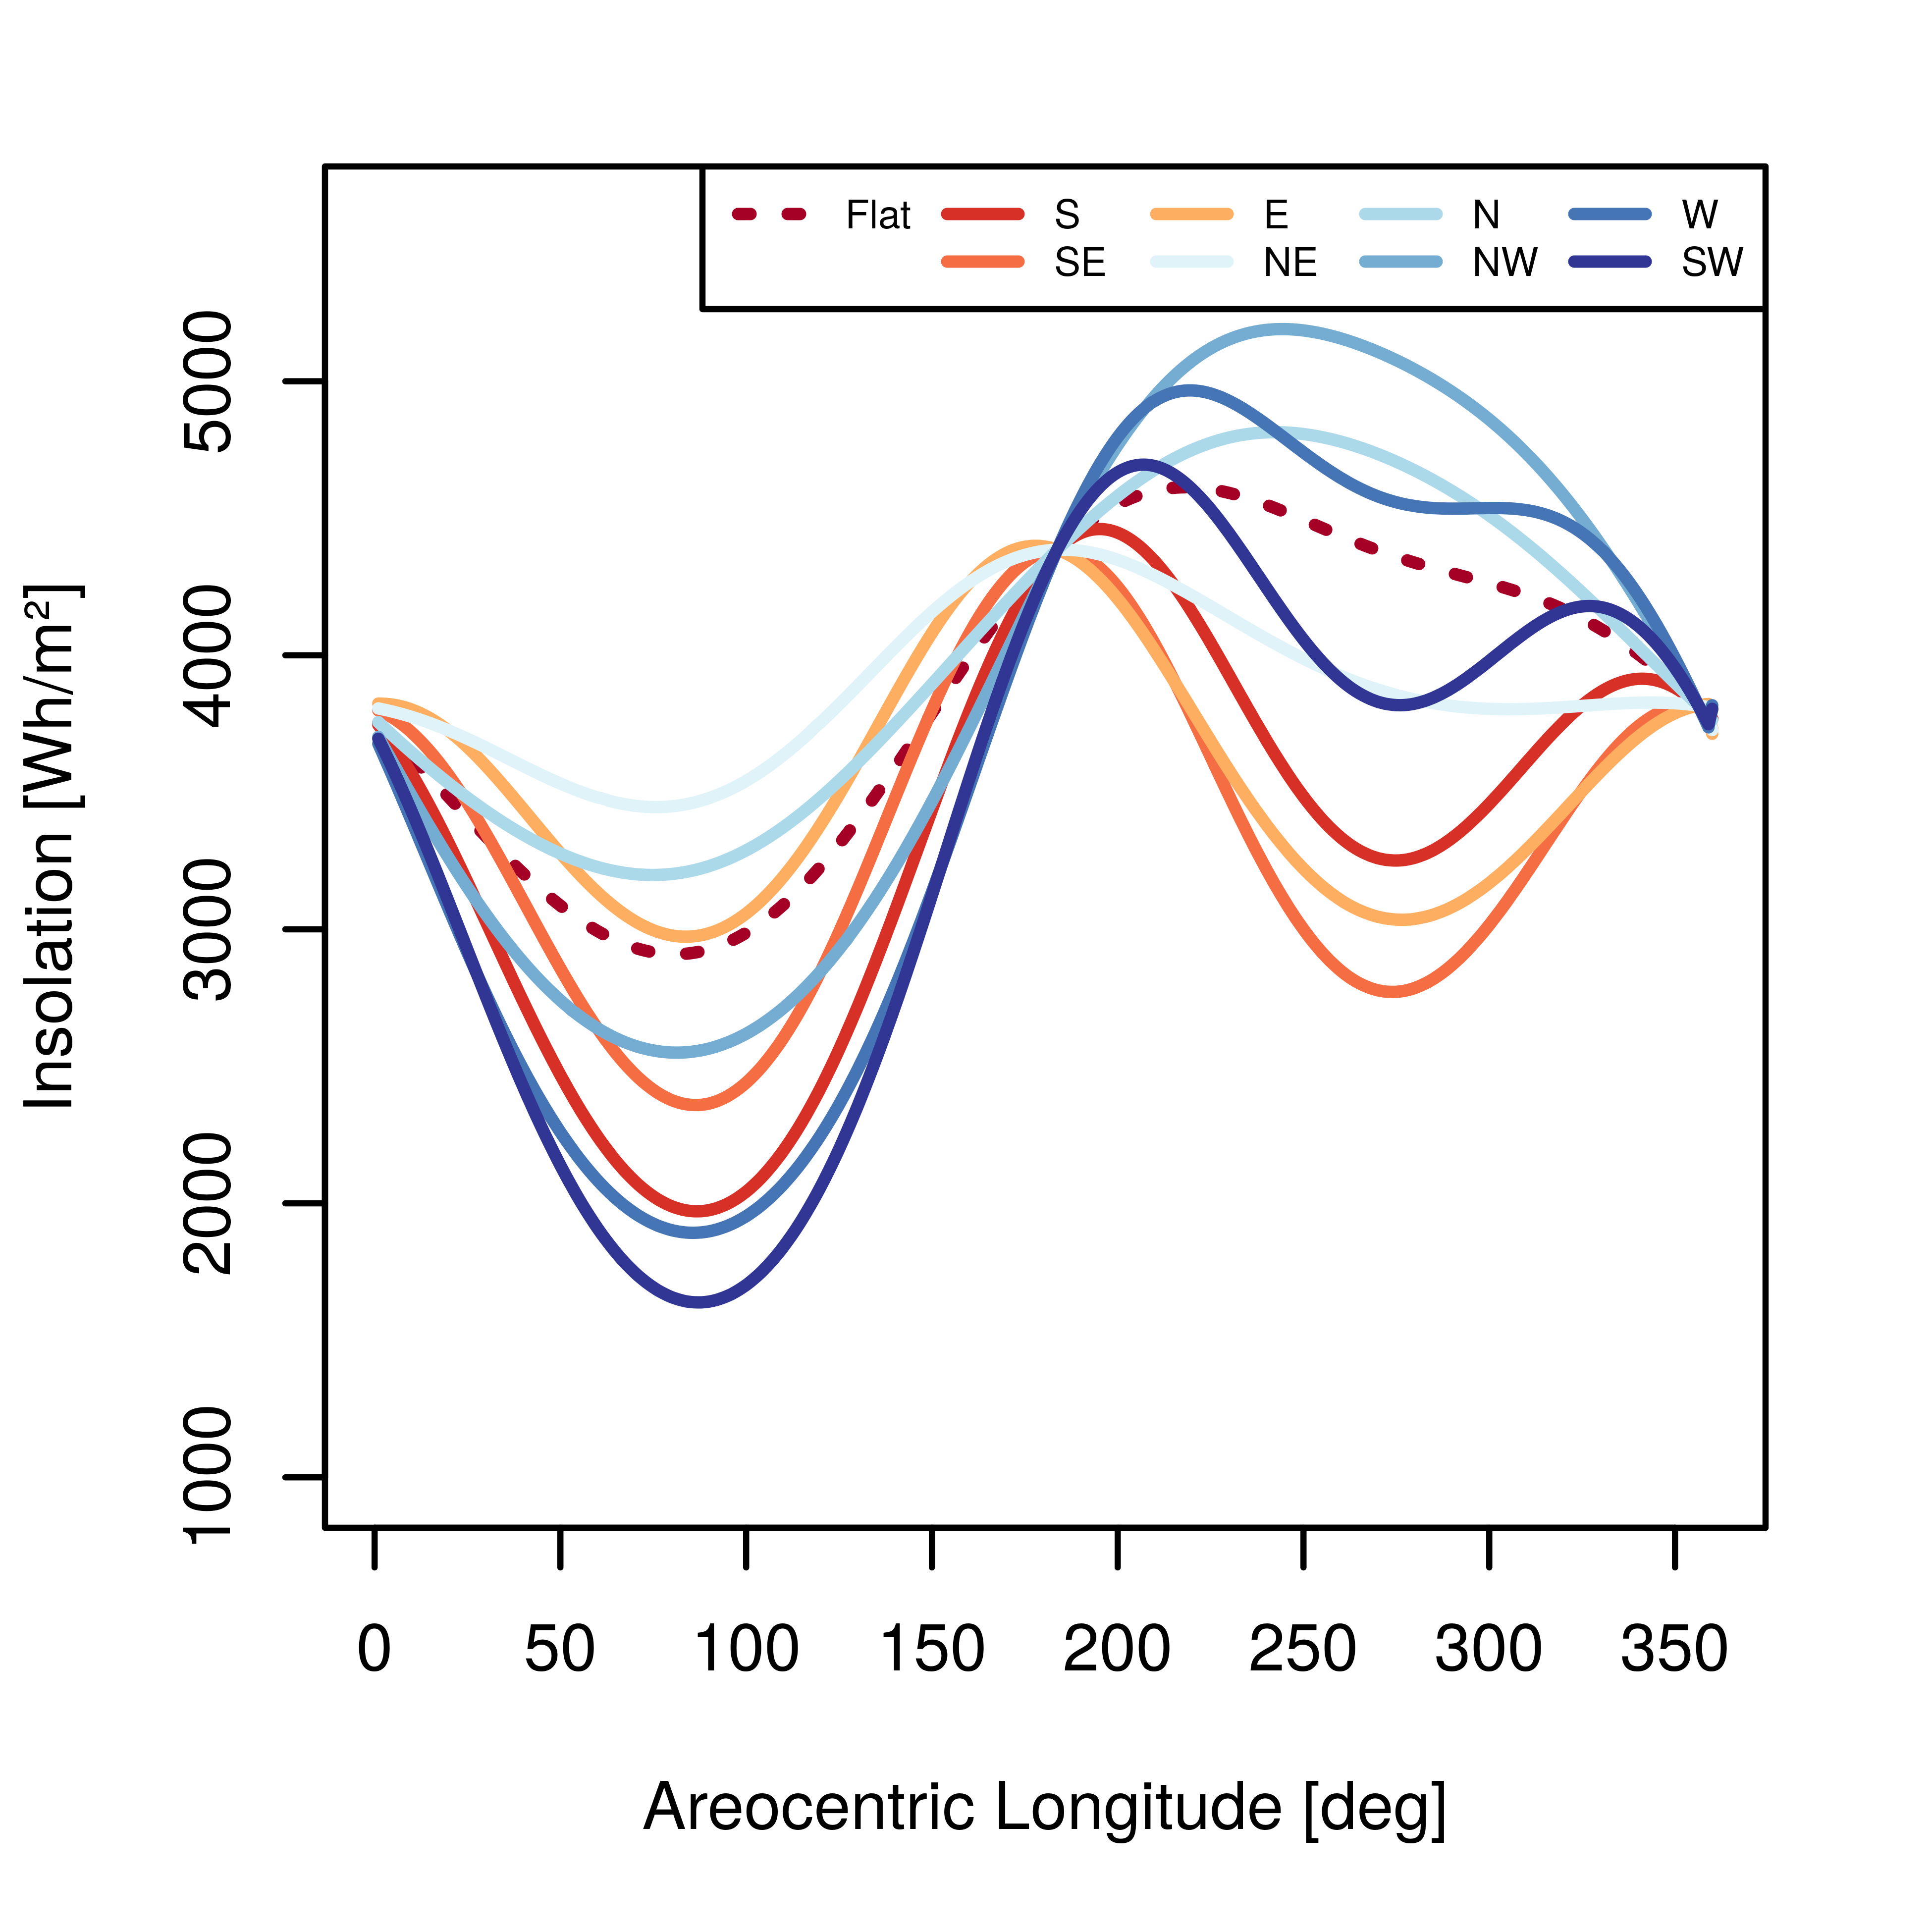
\includegraphics[height=\graphicsHeight]{sections/appendix/optimal-angles/plots/iani-chaos-tau-04-and-beta-optimal-based-on-solar-insolation.png}
            \subcaption{Based on the daily beam insolation on the surface from sunrise to sunset.}
            \label{fig:sub:optimal-angles-iani-chaos-based-on-insolation}
    \end{subfigure}\\[0.8ex]
    \caption[Daily insolation at Iani Chaos with optimal angles $\beta$ for difference orientation angles $\gamma_c$]
    {Daily insolation at Iani Chaos with optimal angles $\beta$ for difference orientation angles $\gamma_c$. Iani Chaos is located in the Sourthern hemisphere at latitude \SI{2}{\degree}S.}
    \label{fig:plot:optimal-angles-iani-chaos}
\vspace{-2ex}
\end{figure}

\clearpage

Figures \ref{fig:plot:optimal-angles-iani-chaos} and \ref{fig:plot:optimal-angles-ismenius-cavus} plot the resulting insolation throughout a Martian year for the calculated optimal $\beta$ angles with different $\gamma_{c}$ angles at Iani Chaos and Ismenius Cavus. Insolations obtained from a flat surface are also included as a reference.

\begin{figure}[h]
\vspace{-2ex}
\centering
    %% setup sizes
    \setlength{\subfigureWidth}{0.50\textwidth}
    \setlength{\graphicsHeight}{80mm}
    %% kill hyper-link highlighting
    \hypersetup{hidelinks=true}%
    %% the figures
    \begin{subfigure}[t]{\subfigureWidth}
        \centering
            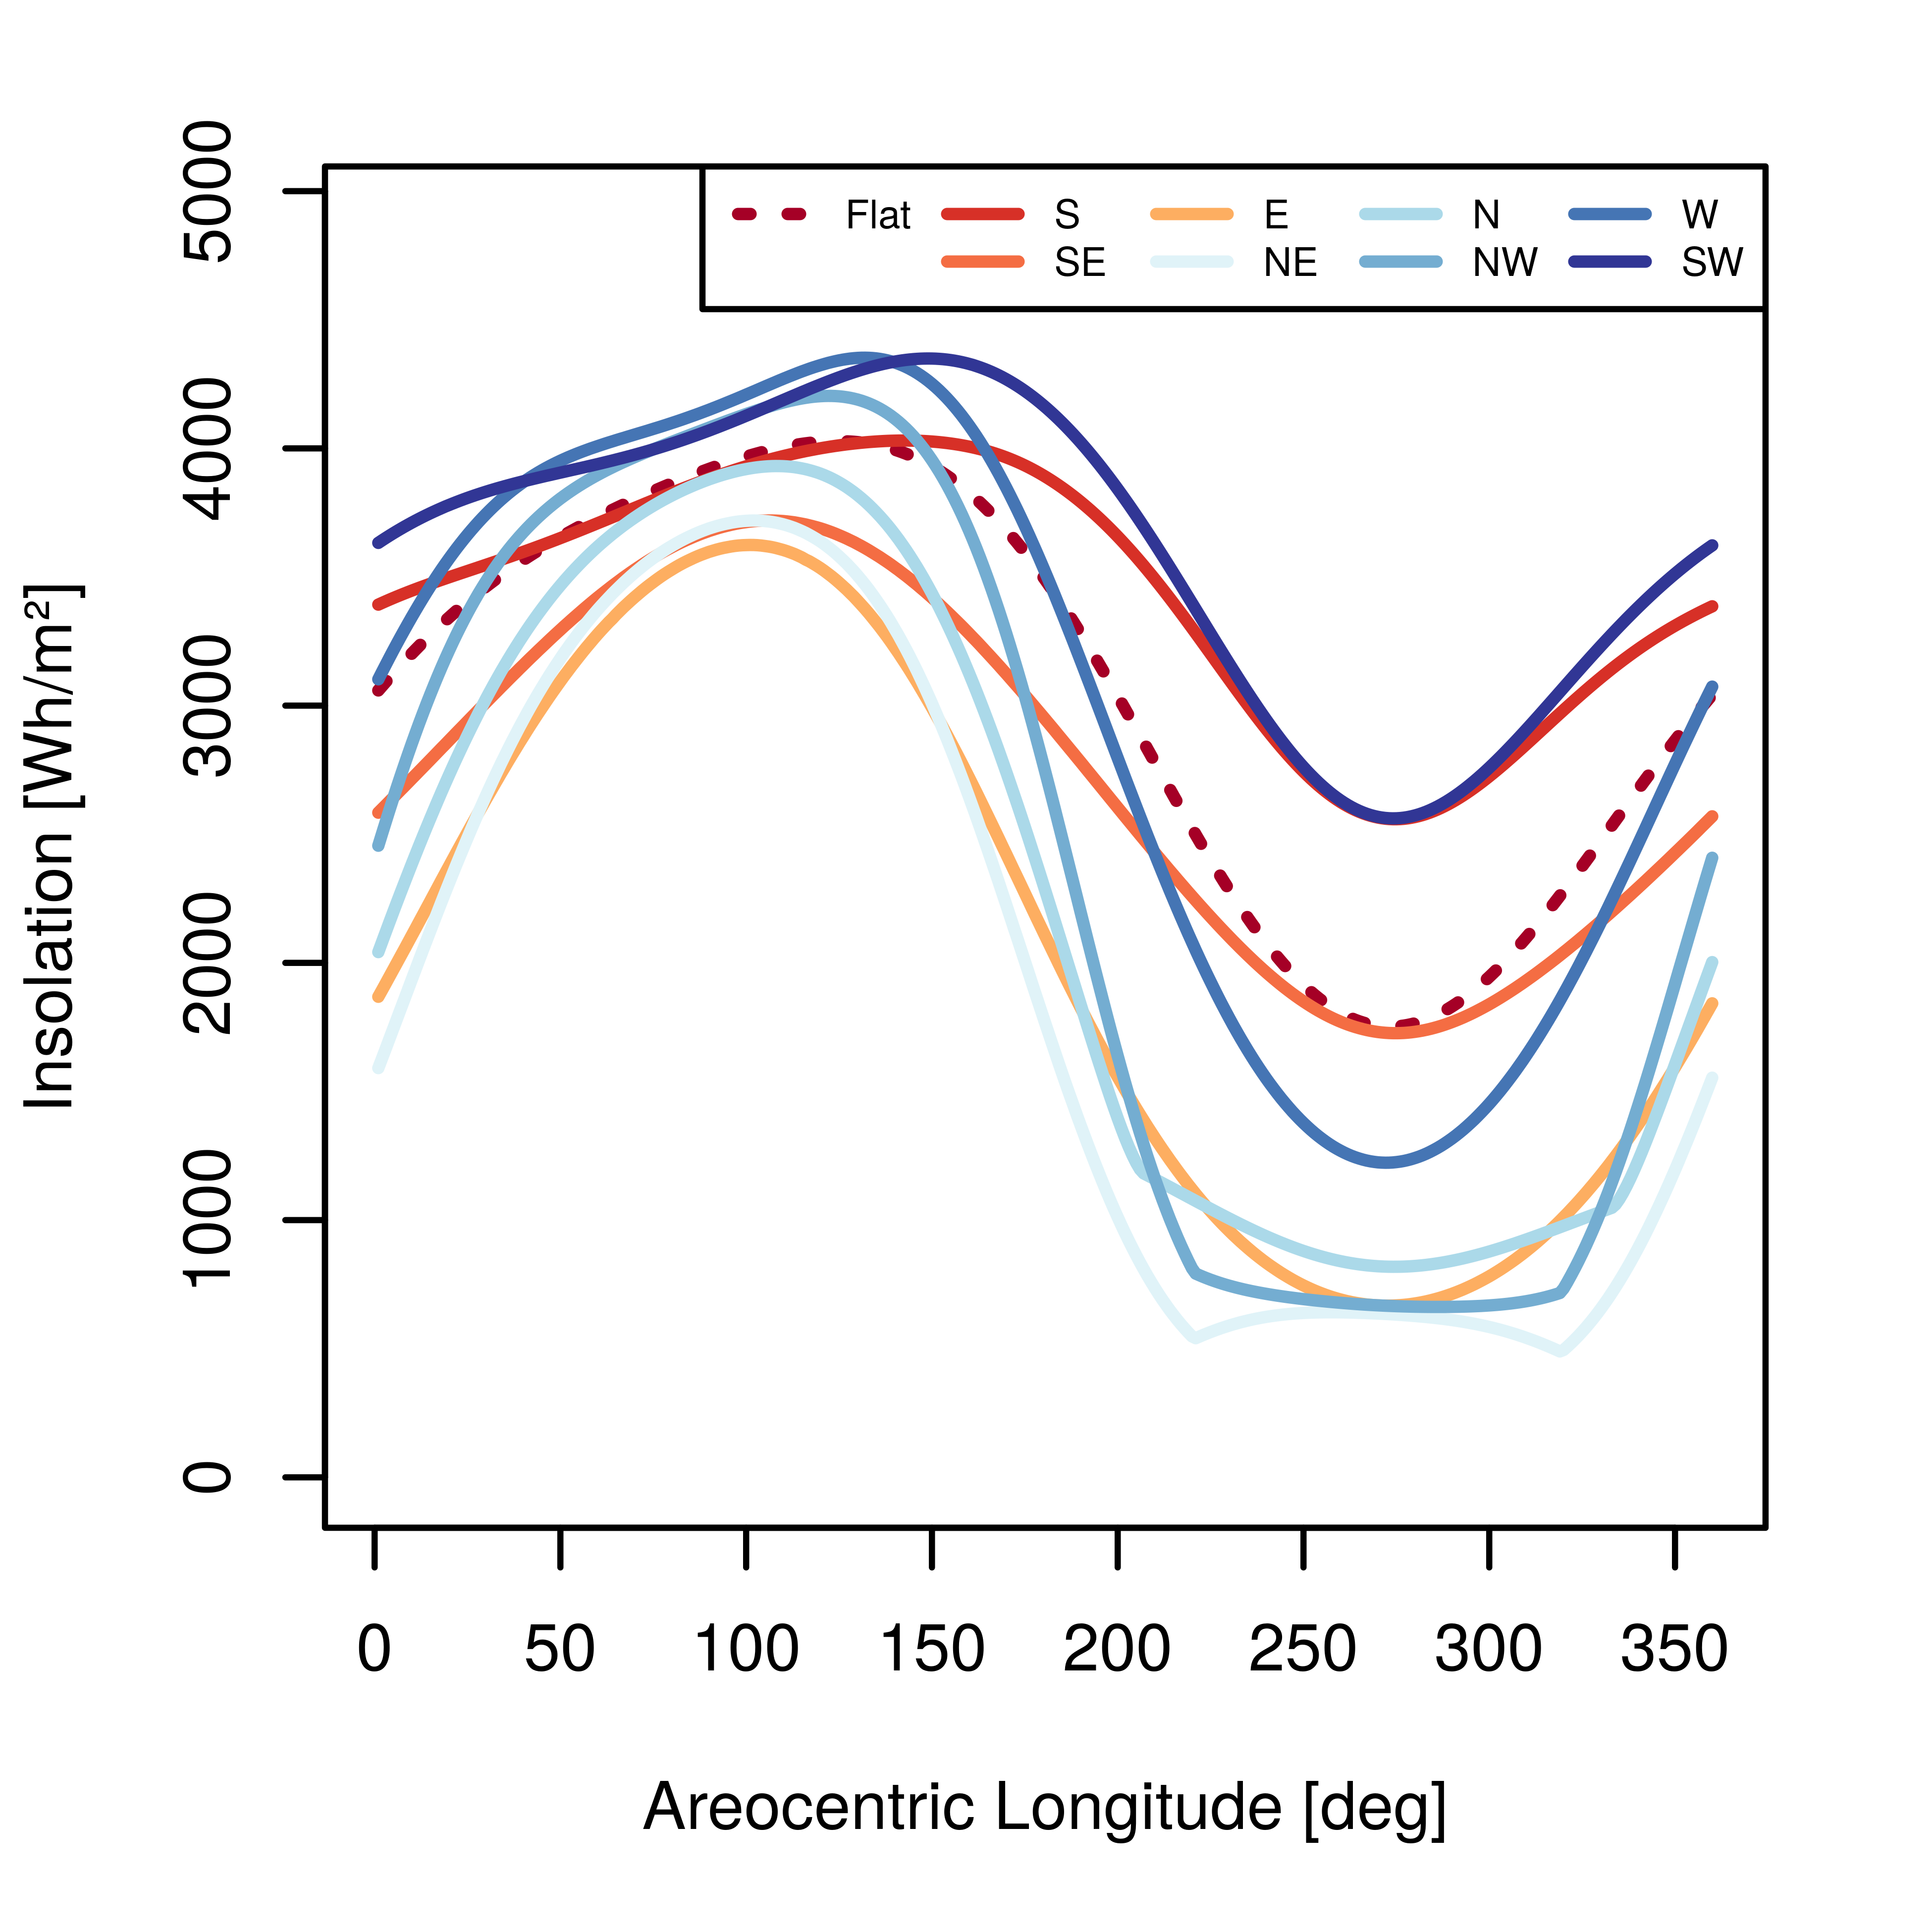
\includegraphics[height=\graphicsHeight]{sections/appendix/optimal-angles/plots/ismenius-cavus-tau-04-and-beta-optimal-based-on-direct-beam-irradiance-at-noon.png}
            \subcaption{Based on the direct beam irradiance at noon.}
            \label{fig:sub:optimal-angles-ismenius-cavus-based-on-irradiance}
    \end{subfigure}\hfill
    \begin{subfigure}[t]{\subfigureWidth}
        \centering
            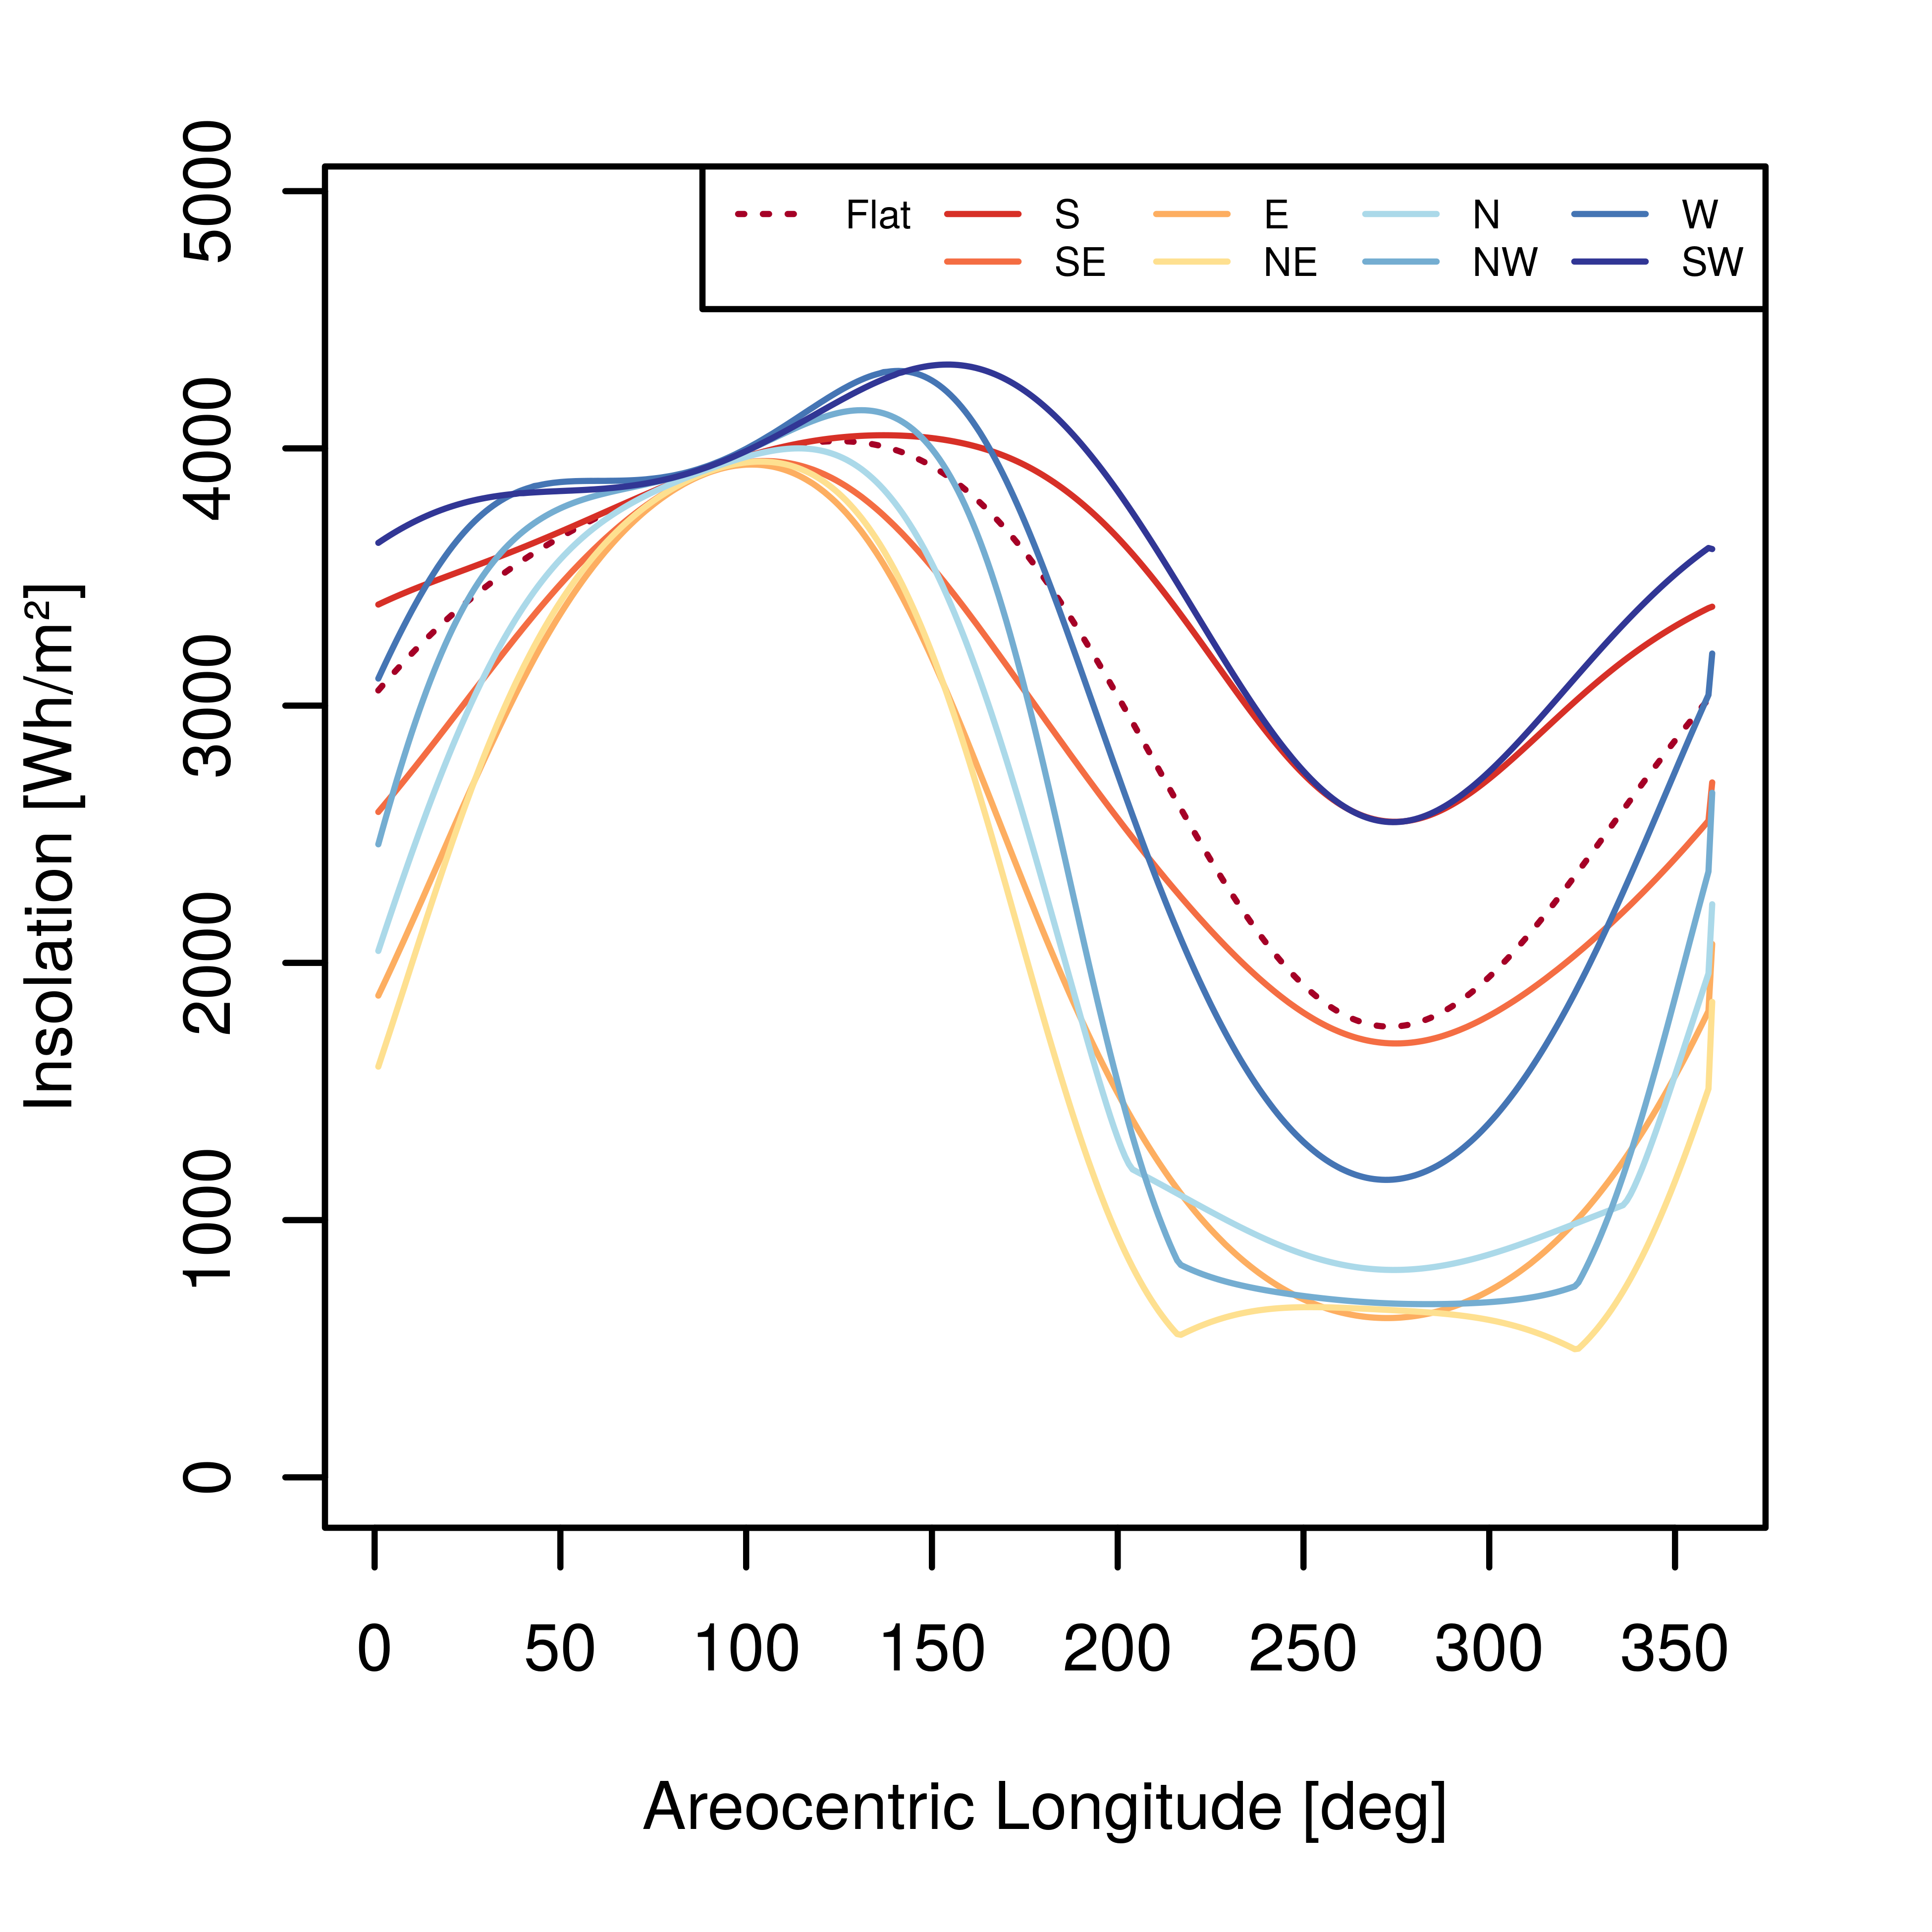
\includegraphics[height=\graphicsHeight]{sections/appendix/optimal-angles/plots/ismenius-cavus-tau-04-and-beta-optimal-based-on-solar-insolation.png}
            \subcaption{Based on the daily beam insolation on the surface from sunrise to sunset.}
            \label{fig:sub:optimal-angles-ismenius-cavus-based-on-insolation}
    \end{subfigure}\\[0.8ex]
    \caption[Daily insolation at Ismenius Cavus with optimal angles $\beta$ for difference orientation angles $\gamma_c$]
    {Daily insolation at Ismenius Cavus with optimal angles $\beta$ for difference orientation angles $\gamma_c$. Ismenius Cavus is located in the Northern hemisphere at latitude \SI{34}{\degree}N.}
    \label{fig:plot:optimal-angles-ismenius-cavus}
\vspace{-2ex}
\end{figure}

The results suggest that the optimal pairing between $\gamma_{c}$ and $\beta$ differs than what is calculated with Equations \ref{eq:optimal_beta_irradiance} and \ref{eq:optimal_beta_insolation}.

At Iani Chaos, in the Southern hemisphere, Figure \ref{fig:sub:optimal-angles-iani-chaos-based-on-irradiance} suggests that a South East orientation is optimal during Autumn and Winter season until approximately the Vernal Equinox ($L_{s} = \SI{180}{\degree}$) from which point a South West orientation is preferred for the Spring and Summer seasons. However, Figure \ref{fig:sub:optimal-angles-iani-chaos-based-on-insolation} suggests Northward orientation during Autumn and Winter seasons, preserving a flat surface around the Vernal Equinox, and a South West orientation during the Spring and Summer seasons.

At Ismenius Cavus, in the Northern hemisphere, Figure \ref{fig:sub:optimal-angles-ismenius-cavus-based-on-irradiance} suggests that a South West orientation is mostly optimal during the entire year wherease Figure \ref{fig:sub:optimal-angles-ismenius-cavus-based-on-insolation} suggests
